\chapter{GPU implementation}

This chapter guides the reader through the implementation of Mahalanobis based hierarchical clustering analysis. First, we describe the algorithm and high level look on implementation. Then, we thoroughly describe the most important functions.

\section{CUDA}

The problem this chapter aims to solve is implementing an aplication that is able to provide hierarchical clustering of very large datasets while retaining the reasonable computation time --- the time required to compute by a magnitude smaller datasets with current HCA algorithms.
Trying to achive this performance, we used a combination of C++ programming language and \textbf{CUDA}\footnote{Compute Unified Device Architecture.} API.  

CUDA is a parallel platform with API allowing a programmer to use GPU for general purpose programming. This API exposes computational power of hundreds (even thousands) cores of CUDA-enabled GPUs.


\subsection{Terminology}

The starting point for running any code on GPU using CUDA is a \textbf{kernel}. A~kernel is a function that is executed on GPU; we say it contains \emph{device code}. Complementary to a device code, a \emph{host code} is the phrase for code executed on CPU. Hence, a common CUDA application runs host code that determines which device code to run next. 

Kernel is run $n$ times in parallel by $n$ threads each having its unique \emph{thread ID}. IDs of threads can be identified by \emph{one-dimensional}, \emph{two-dimensional} or \emph{three-dimensional} indices forming block of threads, called \textbf{thread block}. This property reflects shapes of common structures such as vectors and matrices resulting in natural computation.

Since all block threads reside on the same processor and share common resources, the block size is limited\footnote{Currently up to 1024 threads.}. However, a kernel can be launched with multiple equally shaped blocks to increase the number of running threads. They can be organised into up to three-dimensional structure called \textbf{grid}. This naturally implies unique block ID. A grid can be of an arbitrary size; usually dictated by the computed data. It is a common practise that grid size surpasses the number of GPU processors.


The device memory is hierarchicaly divided into parts each being accessible by a different set of threads:
\begin{description}
	\item[Global memory] -- This memory is accessible by any thread. Any memory request is transfered via tranactions; hence, to avoid reduction of throughput, memory accesses should be coalesced. 
	\item[Local memory] -- Each thread has exclusive access to its local memory. Do not mislead this with registers, local memory is a private global memory.
	\item[Shared memory] -- Shared memory is assigned to a block, meaning that threads from the same block has access to the same shared memory. It is placed on-chip so it has much lower latency and higher bandwith than the global or local memory.
	\item[Constant memory] -- Read only memory accesible by any thread. Due to its read-only property, it can be heavily cached. Together with global memory, it persists across different kernel launches.
\end{description}

\begin{figure}\centering
	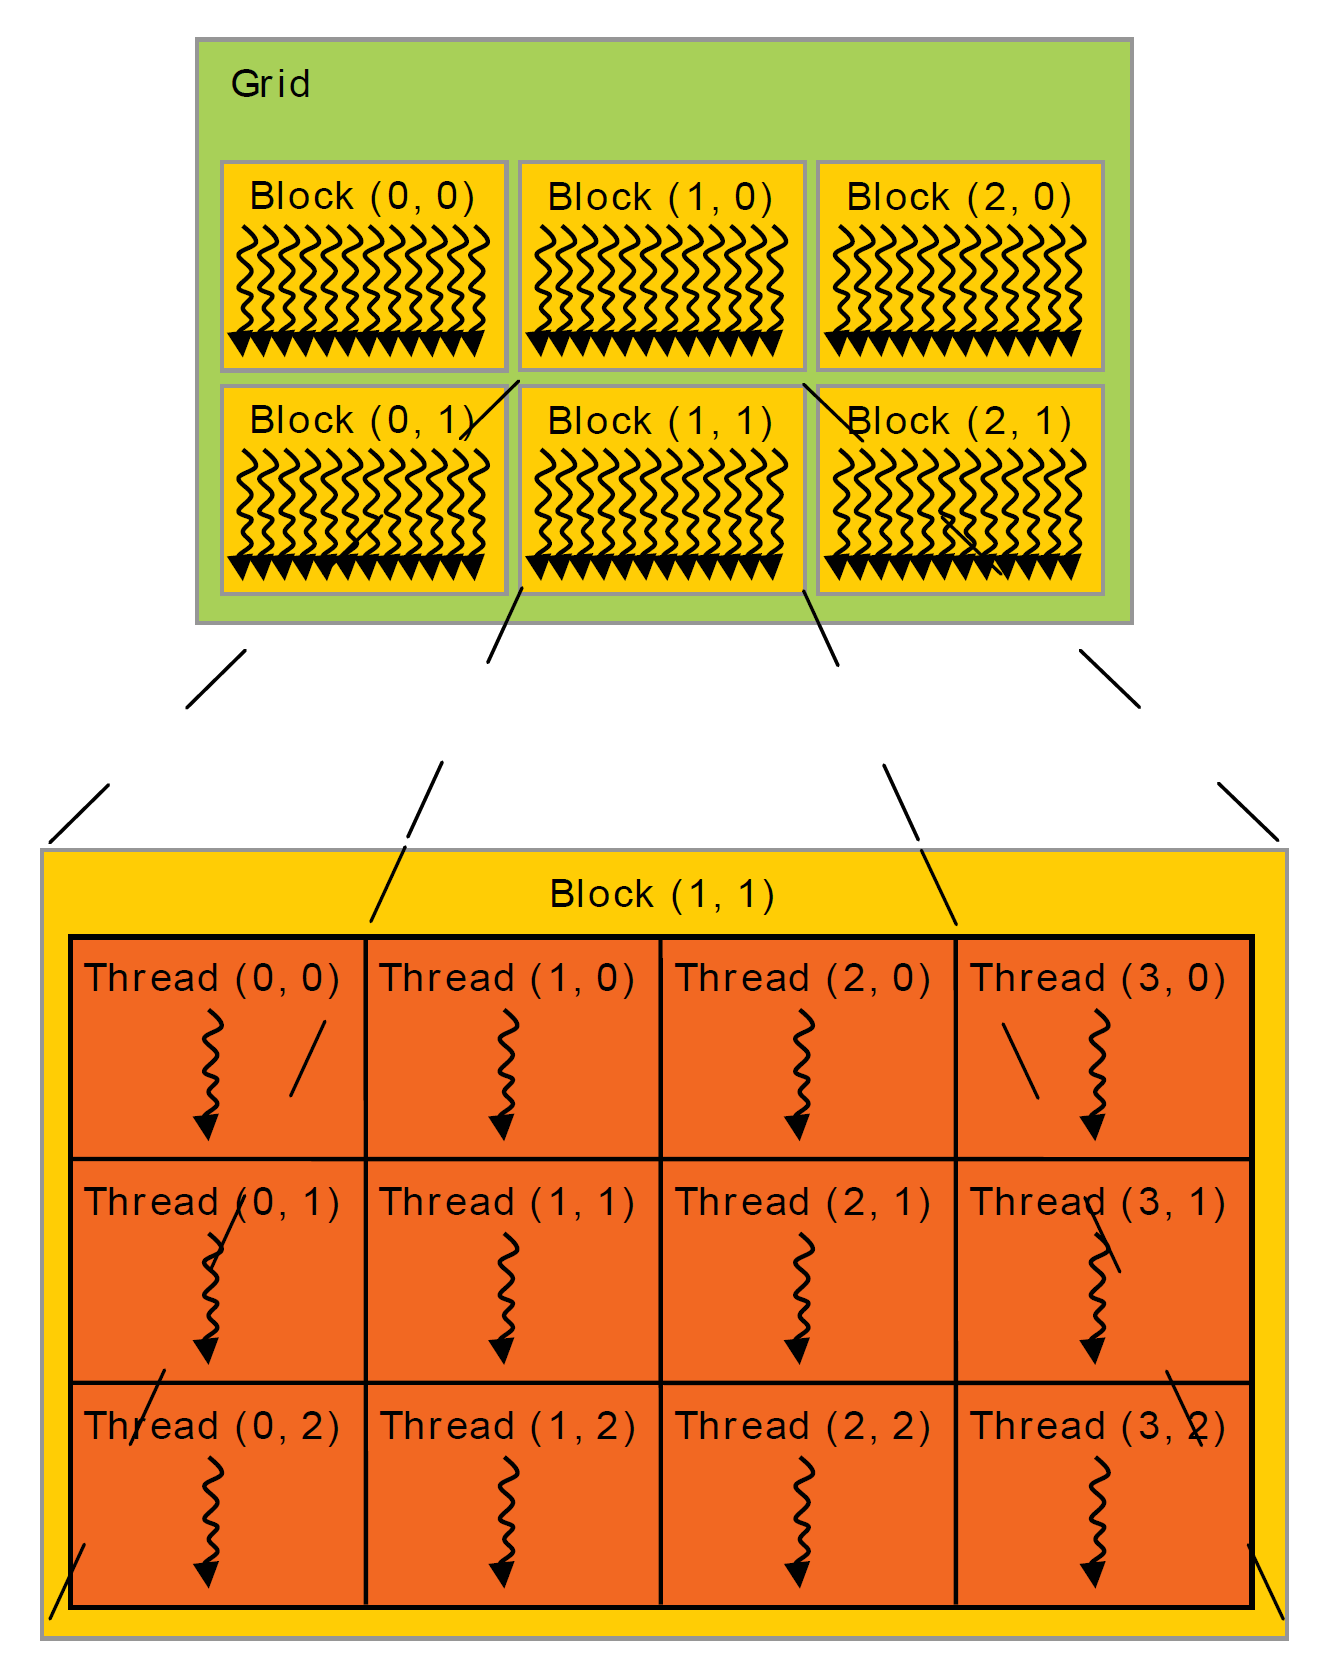
\includegraphics[width=8cm]{img/grid}
	\caption{Example of 2D grid of size (3,2) with 2D blocks of size (4,3).}
	\label{fig02:grid}
\end{figure}

\subsection{GPU Architecture}

To dive deeper into describing each parallel piece of code run on GPU, we describe CUDA-enabled GPU architecture to lay foundation for the further terminology.
\begin{description}
	\item[Core] is the smallest possible block in the architecture. It has pool of registers and executes single thread.
	\item[Streaming Multiprocessor] is a collection of \emph{cores} organized in a grid-like pattern.
\end{description}

\section{specs of machine}

code was optimized for this machine

\section{impl description}

high level look

describe each kernel